\hypertarget{introduction}{%
\section{Introduction}\label{introduction}}

Automated Essay Scoring (AES) is the task of assigning a score to
free-form text (throughout this paper essay will be defined loosely to
include short answers) using a computational system. The goal of AES is
to mimic human scoring as closely as possible. The development of the
Transformer in {[}1{]} has significantly improved the performance of
Natural Language Processing (NLP) models to a point where it is
achievable to use a purely neural approach to AES {[}2{]}. This has
created the possibility for many task-agnostic architectures and
pre-training approaches which then allows for greater flexibility in the
implementation of these models. This also makes the cutting-edge
performance of these NLP models available for simple implementation in
real world situations.

Transformer models such as those in {[}1{]}, {[}3{]}, {[}4{]} and many
more have the significant disadvantage that they require a very large
training dataset and high training time to achieve decent performance.
This makes training these models from scratch almost unachievable for
most tasks (which don't have very large datasets available). A good
solution to this is pre-training where the model is first trained by the
creator on a task-agnostic dataset and, if necessary, the model can then
be fine-tuned to the downstream task that it will be applied to. After
fine-tuning these models can achieve the performance increase of a
transformer model with minimal training time and a small training
dataset.

All sequence to sequence transformer models use an encoder-decoder
architecture where the input sequence is fed into an encoder. The
encoder then outputs a vector or matrix representation of the input
sequence known as the `hidden vector' or `hidden matrix'. This can then
be inputted into a decoder which converts this hidden data back into an
output sequence. Since the encoder and decoder are independent networks,
the decoder can be replaced with a classification or regression head,
taking the hidden data as its input and outputting multiple or a single
neuron value. This significantly expands the tasks transformers can be
applied to.

The encoders and decoders do not have to use a transformer architecture,
they can be replaced by older Recurrent Neural Networks (RNNs). Even
though RNNs often perform worse than transformer models, on small
datasets they do often perform similarly or better than transformer
models (even if the transformer is pre-trained).

For the task of AES there has been discussion on whether a
classification approach is better than a regression approach (and vice
versa) {[}5{]}. It was found that a regression approach performs better
for their dataset, however, if a pre-training approach is used for an
AES system classification has the significant disadvantage that the
number of marks given cannot be changed between the pre-training step
and the fine-tuning step, whereas with a regression approach the number
of marks is irrelevant which may significantly improve the size of the
dataset that can be used, or even if a pre-training approach is
reasonable.

The distribution of scores given to a set of essays is naturally very
unbalanced as the aim for human markers is often to obtain a normal
distribution of the scores. This means that there are few answers that
achieve the very worst scores and very few that achieve the highest
scores. Unbalanced datasets can significantly reduce the performance of
a classification model. Unbalanced datasets can pose an issue for a
regression model in that it can be easier for the model to only predict
the mean of the training data, this is a significant problem for AES as
it is very important that each sample is given as accurate a score as
possible. The loss function proposed in this paper aims to solve this
problem.

\hypertarget{dataset}{%
\section{Dataset}\label{dataset}}

The dataset used to train this model was introduced in the Kaggle
Automated Student Assessment Prize (ASAP) in 2012.\footnote{\url{https://kaggle.com/c/asap-aes}}
For the ASAP competition two datasets were introduced, one containing
essays (approx. 150-650 words) and the other containing short answers
(\textless{} 100 words). This model is trained only on the essay
dataset. Table \ref{tbl:asap-aes} shows the details of the dataset.

\begin{longtable}[]{@{}
  >{\raggedright\arraybackslash}p{(\columnwidth - 4\tabcolsep) * \real{0.2222}}
  >{\raggedright\arraybackslash}p{(\columnwidth - 4\tabcolsep) * \real{0.2500}}
  >{\raggedright\arraybackslash}p{(\columnwidth - 4\tabcolsep) * \real{0.2917}}@{}}
\caption{ASAP AES dataset \label{tbl:asap-aes}}\tabularnewline
\toprule()
\begin{minipage}[b]{\linewidth}\raggedright
Prompt
\end{minipage} & \begin{minipage}[b]{\linewidth}\raggedright
No.~of Samples
\end{minipage} & \begin{minipage}[b]{\linewidth}\raggedright
Score Range
\end{minipage} \\
\midrule()
\endfirsthead
\toprule()
\begin{minipage}[b]{\linewidth}\raggedright
Prompt
\end{minipage} & \begin{minipage}[b]{\linewidth}\raggedright
No.~of Samples
\end{minipage} & \begin{minipage}[b]{\linewidth}\raggedright
Score Range
\end{minipage} \\
\midrule()
\endhead
1 & 1,783 & 2-12 \\
2 & 1,800 & 1-6 \\
3 & 1,726 & 0-3 \\
4 & 1,772 & 0-3 \\
5 & 1,805 & 0-4 \\
6 & 1,800 & 0-4 \\
7 & 1,569 & 0-30 \\
8 & 723 & 0-60 \\
\bottomrule()
\end{longtable}

The model was trained on each prompt individually. First the dataset is
shuffled with 90\% of the data used for training and the other 10\% used
for evaluation.

\hypertarget{model}{%
\section{Model}\label{model}}

\hypertarget{architecture}{%
\subsection{Architecture}\label{architecture}}

The model used in this paper is a Long Short-Term Memory (LSTM) {[}6{]}
encoder using an attention mechanism {[}7{]}. The regression head used
for this model is a single fully connected layer where the hidden data
is inputted and a single value is outputted.

To tokenise the input sequence the same tokeniser used in the BERT model
{[}3{]} is used. This choice was made because the BERT tokeniser
tokenises on word-parts rather than whole words. This allows the model
to be more confident in the meaning of words that are not in its
original training data, which may occur when using technical language in
an essay.

\begin{figure}[h!]
\centering
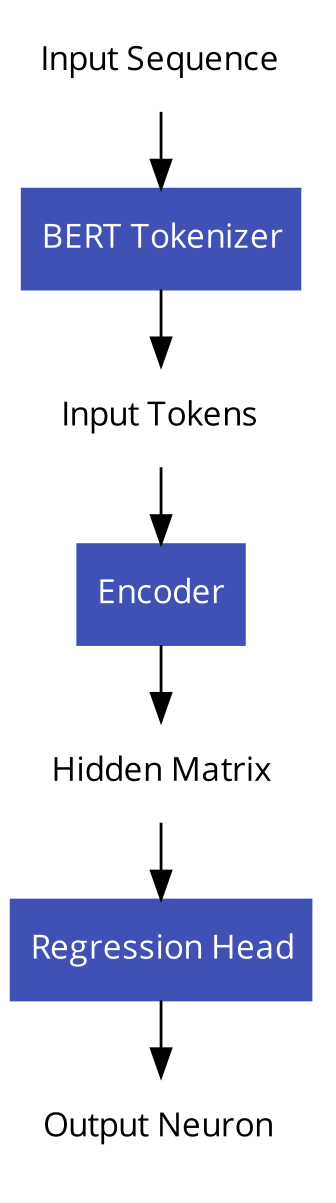
\includegraphics[height=8cm]{../model-basic}
\caption{Model architecture}
\label{fig:arch}
\end{figure}

\begin{figure}[h!]
\centering
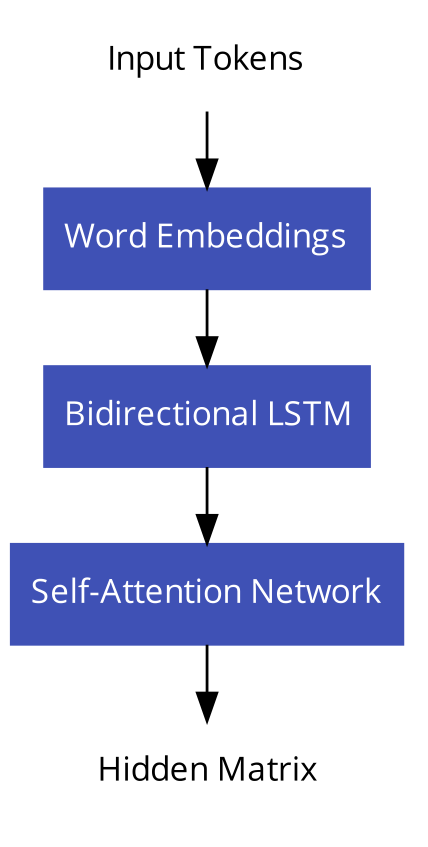
\includegraphics[height=6cm]{../encoder}
\caption{Encoder architecture}
\label{fig:encoder}
\end{figure}

Fig. \ref{fig:arch} shows the flow of data through the model and Fig.
\ref{fig:encoder} takes a closer look at the architecture of the
encoder.\footnote{Images created with
  \href{https://code2flow.com}{code2flow}}

\hypertarget{metrics}{%
\subsection{Metrics}\label{metrics}}

In the ASAP competition the metric used was the Quadratic Weighted Kappa
(QWK) defined in {[}8{]}.

The model was also evaluated on Mean Squared Error (MSE), defined in Eq.
\ref{eq:mse}, Mean Absolute Error (MAE), defined in Eq. \ref{eq:mae} and
the coefficint of determination \(r^2\), defined in Eq. \ref{eq:r2}.

\begin{equation} \text{MSE}(\mathbf{x}, \mathbf{y}) = \frac{1}{N} \sum^{N}_{i=0} (y_i-x_i)^2 \label{eq:mse}\end{equation}

\begin{equation} \text{MAE}(\mathbf{x}, \mathbf{y}) = \frac{1}{N} \sum^N_{i=0} |y_i-x_i| \label{eq:mae}\end{equation}

\begin{equation} r^2 = 1-\frac{\sum^N_{i=0} (y_i-x_i)^2}{\sum^N_{i=0} (y_i-\bar{y})} \label{eq:r2}\end{equation}

where \(\mathbf{x}\) are the true values, \(\mathbf{y}\) are the
predicted values, \(N\) is the number of samples and \(\bar{y}\) is the
mean predicted value.

\hypertarget{the-dynamic-loss-function}{%
\section{The dynamic loss function}\label{the-dynamic-loss-function}}

A loss function is the function that is minimized during the training of
the network. The aim of a loss function is to determine the difference
between what the models outputs are and what they should be. A dynamic
loss function is when the loss function is changed throughout the
training process. The main benefit of a dynamic loss function is the
ability to adjust the goals of the model at different times during the
training process.

A common problem with regression models is that the model tends towards
predicting the mean of the training dataset with very little variation.
This can occur when the dataset is unbalanced (as is often the case with
real world datasets), however, in prior testing it did occur on the ASAP
AES dataset.

A solution to this problem is to adjust the loss function to provide an
incentive to predicting batches with the correct sample standard
deviation. Do do this, a loss function can be defined as the error in
the standard deviation of a certain batch:

\begin{equation} \text{STDE}(\mathbf{x}, \mathbf{y}) = |\sigma(\mathbf{y})-\sigma(\mathbf{x})| \label{eq:stderror}\end{equation}

where \(\sigma\) is the function calculating the sample standard
deviation.

Multiple loss functions can be combined using a weighted sum, and some
constant \(p\):

\begin{equation} L_T = pL_1 + (1-p)L_2 \label{eq:combine-loss}\end{equation}

where \(L_T\) is the total loss and \(L_1\) and \(L_2\) are two loss
functions.

Therefore, using \(\text{STDE}\) as \(L_1\) and \(\text{MSE}\) as
\(L_2\) a loss function is defined that provides an incentive to predict
using the correct standard deviation and with minimal error.

Using a constant value of \(p\) did help to prevent this form of
underfitting, however, the model was still showing significant
underfitting and because of the reduced importance of an error metric
the model's performance was significantly reduced. In an attempt to
solve both of these problems, the value of \(p\) could be decayed over
time using an exponential decay function (shown in Eq. \ref{eq:decay}).
When the decay was started as soon as the training began it was found
that the model would still show signs of underfitting, this could easily
be solved by holding \(p\) constant for the first portion of training
and then decaying its value throughout the rest of the training process.
The full definition of \(p\) as a function of training step or epoch is
shown in Eq. \ref{eq:min-decay}.

\begin{equation} p(t) = a\cdot \exp\left(-\frac{t}{T}\right) \label{eq:decay}\end{equation}

\begin{equation} p(t) = \min\left(a, a \cdot \exp\left(-c\left(\frac{t}{T}-b\right)\right)\right) \label{eq:min-decay}\end{equation}

where \(t\) is the current training step or current epoch, \(T\) is the
total number of training step or total number of training epochs and
\(a\), \(b\) and \(c\) are constants. Fig. \ref{fig:p} shows an example
plot of \(p\) against fraction of training complete.

\begin{figure}[h!]
\centering
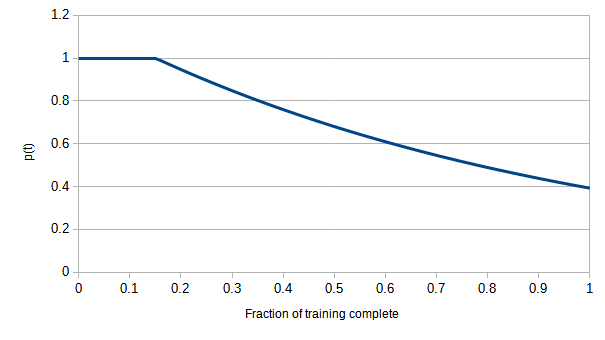
\includegraphics[height=6cm]{p-value}
\caption{Value of $p$ against fraction of training complete using $a=1$, $b=0.15$ and $c=1.1$}
\label{fig:p}
\end{figure}

This method achieved the highest performance without sacrificing either
metric.

\hypertarget{results}{%
\section{Results}\label{results}}

\begin{table}[H]
\caption{Our system compared to EASE and Tahipour \& Ng's LSTM model with Mean over Time}
\begin{tabular}{|l|llllll|}
\hline
\multirow{2}{*}{System} & \multicolumn{6}{c|}{Prompt}                                                                                                                              \\ \cline{2-7} 
                        & \multicolumn{1}{l|}{1}     & \multicolumn{1}{l|}{4}     & \multicolumn{1}{l|}{5}     & \multicolumn{1}{l|}{6}     & \multicolumn{1}{l|}{7}     & Avg QWK \\ \hline
Ours                    & \multicolumn{1}{l|}{0.841} & \multicolumn{1}{l|}{0.773} & \multicolumn{1}{l|}{0.807} & \multicolumn{1}{l|}{0.739} & \multicolumn{1}{l|}{0.765} & 0.788   \\ \hline
EASE (SVR)              & \multicolumn{1}{l|}{0.781} & \multicolumn{1}{l|}{0.749} & \multicolumn{1}{l|}{0.782} & \multicolumn{1}{l|}{0.771} & \multicolumn{1}{l|}{0.727} & 0.763   \\ \hline
EASE (BLRR)             & \multicolumn{1}{l|}{0.761} & \multicolumn{1}{l|}{0.742} & \multicolumn{1}{l|}{0.784} & \multicolumn{1}{l|}{0.775} & \multicolumn{1}{l|}{0.730} & 0.759   \\ \hline
Tahipour \& Ng LSTM     & \multicolumn{1}{l|}{0.775} & \multicolumn{1}{l|}{0.795} & \multicolumn{1}{l|}{0.818} & \multicolumn{1}{l|}{0.813} & \multicolumn{1}{l|}{0.805} & 0.802   \\ \hline
\end{tabular}
\end{table}

\hypertarget{references}{%
\section*{References}\label{references}}
\addcontentsline{toc}{section}{References}

\hypertarget{refs}{}
\begin{CSLReferences}{0}{0}
\leavevmode\vadjust pre{\hypertarget{ref-vaswaniAttentionAllYou2017}{}}%
\CSLLeftMargin{{[}1{]} }%
\CSLRightInline{A. Vaswani \emph{et al.}, {``Attention {Is All You
Need},''} p. 11, 2017.}

\leavevmode\vadjust pre{\hypertarget{ref-ludwigAutomatedEssayScoring2021}{}}%
\CSLLeftMargin{{[}2{]} }%
\CSLRightInline{S. Ludwig, C. Mayer, C. Hansen, K. Eilers, and S.
Brandt, {``Automated {Essay Scoring Using Transformer Models},''}
\emph{Psych}, vol. 3, no. 4, pp. 897--915, Dec. 2021, doi:
\href{https://doi.org/10.3390/psych3040056}{10.3390/psych3040056}.}

\leavevmode\vadjust pre{\hypertarget{ref-devlinBERTPreTrainingDeep2019}{}}%
\CSLLeftMargin{{[}3{]} }%
\CSLRightInline{J. Devlin, M.-W. Chang, K. Lee, and K. Toutanova,
{``{BERT}: {Pre-Training} of {Deep Bidirectional Transformers} for
{Language Understanding},''} \emph{arXiv:1810.04805 {[}cs{]}}, May 2019,
Available: \url{https://arxiv.org/abs/1810.04805}}

\leavevmode\vadjust pre{\hypertarget{ref-beltagyLongformerLongDocumentTransformer2020}{}}%
\CSLLeftMargin{{[}4{]} }%
\CSLRightInline{I. Beltagy, M. E. Peters, and A. Cohan, {``Longformer:
{The Long-Document Transformer},''} \emph{arXiv:2004.05150 {[}cs{]}},
Dec. 2020, Available: \url{https://arxiv.org/abs/2004.05150}}

\leavevmode\vadjust pre{\hypertarget{ref-johanberggrenRegressionClassificationAutomated2019}{}}%
\CSLLeftMargin{{[}5{]} }%
\CSLRightInline{S. Johan Berggren, T. Rama, and L. Øvrelid,
{``Regression or {Classification}? {Automated Essay Scoring} for
{Norwegian},''} in \emph{Proceedings of the {Fourteenth Workshop} on
{Innovative Use} of {NLP} for {Building Educational Applications}},
2019, pp. 92--102. doi:
\href{https://doi.org/10.18653/v1/W19-4409}{10.18653/v1/W19-4409}.}

\leavevmode\vadjust pre{\hypertarget{ref-hochreiterLongShortTermMemory1997}{}}%
\CSLLeftMargin{{[}6{]} }%
\CSLRightInline{S. Hochreiter and J. Schmidhuber, {``Long {Short-Term
Memory},''} \emph{Neural Computation}, vol. 9, no. 8, pp. 1735--1780,
Nov. 1997, doi:
\href{https://doi.org/10.1162/neco.1997.9.8.1735}{10.1162/neco.1997.9.8.1735}.}

\leavevmode\vadjust pre{\hypertarget{ref-bahdanauNeuralMachineTranslation2016b}{}}%
\CSLLeftMargin{{[}7{]} }%
\CSLRightInline{D. Bahdanau, K. Cho, and Y. Bengio, {``Neural {Machine
Translation} by {Jointly Learning} to {Align} and {Translate}.''}
{arXiv}, May 2016. doi:
\href{https://doi.org/10.48550/arXiv.1409.0473}{10.48550/arXiv.1409.0473}.}

\leavevmode\vadjust pre{\hypertarget{ref-taghipourNeuralApproachAutomated2016}{}}%
\CSLLeftMargin{{[}8{]} }%
\CSLRightInline{K. Taghipour and H. T. Ng, {``A {Neural Approach} to
{Automated Essay Scoring},''} in \emph{Proceedings of the 2016
{Conference} on {Empirical Methods} in {Natural Language Processing}},
2016, pp. 1882--1891. doi:
\href{https://doi.org/10.18653/v1/D16-1193}{10.18653/v1/D16-1193}.}

\end{CSLReferences}
